\documentclass[12pt]{article}
\usepackage[a4paper, hmargin={2.5cm, 2.5cm}, vmargin={2.5cm, 2.5cm}]{geometry}

\usepackage[utf8]{inputenc}
\usepackage[english]{babel}
\usepackage{amssymb}
\usepackage{amsfonts}
\usepackage{amsmath}
\usepackage{setspace}
\usepackage{algorithm}
\usepackage[noend]{algpseudocode}

%\usepackage[margin=1in]{geometry}
\usepackage{tikz}
\usetikzlibrary{positioning,shapes, shadows, arrows, automata}
%\usepackage[usenames,dvipsnames]{xcolor}

\usepackage{eso-pic} % \AddToShipoutPicture

\usepackage{graphicx}
\usepackage[hidelinks]{hyperref}
\usepackage{float}
\usepackage[danish]{varioref}
\usepackage{multirow}
\usepackage{hhline}
\usepackage{inconsolata}
\usepackage{etoolbox}

\usepackage{fancyhdr}
\usepackage{listings}

%%%%%%%%%%%%%%%%%%%%%%%%%
%         Colors        %

\definecolor{dark-blue}{HTML}{000080}
\definecolor{dark-green}{HTML}{008000}
\definecolor{pale-purple}{HTML}{94558D}
\definecolor{dark-purple}{HTML}{0000AA}
\definecolor{regular-purple}{HTML}{660099}
\definecolor{magenta}{HTML}{B200B2}
\definecolor{light-gray}{HTML}{FAFAFA}
\definecolor{theorem-gray}{HTML}{F0F0F0}
\definecolor{dark-gray}{HTML}{2D2D2D}
\definecolor{comment}{HTML}{808080}
\definecolor{digit}{HTML}{0000FF}

%                       %
%%%%%%%%%%%%%%%%%%%%%%%%%

%%%%%%%%%%%%%%%%%%%%%%%%%
%        Theorem        %

\usepackage{amsthm}
\usepackage{thmtools}
\theoremstyle{definition}

\declaretheoremstyle[
spaceabove=6pt, spacebelow=6pt,
headfont=\normalfont\bfseries,
notefont=\mdseries, notebraces={(}{)},
bodyfont=\normalfont,
postheadspace=1em,
shaded={bgcolor=theorem-gray}
]{exstyle}

\declaretheoremstyle[
spaceabove=6pt, spacebelow=6pt,
headfont=\normalfont\bfseries,
notefont=\mdseries, notebraces={(}{)},
bodyfont=\normalfont,
postheadspace=1em,
shaded={bgcolor=theorem-gray}
]{defstyle}

%\declaretheorem[thmbox=M]{definition}
\declaretheorem[style=defstyle]{definition}
%\declaretheorem[thmbox=M]{example}
\declaretheorem[style=exstyle]{example}

%                       %
%%%%%%%%%%%%%%%%%%%%%%%%%

%%%%%%%%%%%%%%%%%%%%%%%%%
%   subsubsubsection    %

\usepackage{titlesec}
\titleclass{\subsubsubsection}{straight}[\subsection]

\newcounter{subsubsubsection}[subsubsection]
\renewcommand\thesubsubsubsection{\thesubsubsection.\arabic{subsubsubsection}}

\titleformat{\subsubsubsection}
  {\normalfont\normalsize\bfseries}{\thesubsubsubsection}{1em}{}
\titlespacing*{\subsubsubsection}
{0pt}{3.25ex plus 1ex minus .2ex}{1.5ex plus .2ex}

\makeatletter
\def\toclevel@subsubsubsection{4}
\def\l@subsubsubsection{\@dottedtocline{4}{7em}{4em}}
\makeatother

\setcounter{secnumdepth}{4}
\setcounter{tocdepth}{4}

%                       %
%%%%%%%%%%%%%%%%%%%%%%%%%

%%%%%%%%%%%%%%%%%%%%%%%%%
%          Tikz         %

\tikzset{
  treenode/.style = {align=center, inner sep=0pt, text centered,
    font=\sffamily},
  arn_n/.style = {treenode, circle, black, font=\sffamily\bfseries, draw=white, fill=white, text width=1.5em}
}

%                       %
%%%%%%%%%%%%%%%%%%%%%%%%%

%%%%%%%%%%%%%%%%%%%%%%%%%
%       Algorithm       %

\usepackage{xspace}
\usepackage{algpseudocode}
\newcommand*\Let[2]{\State #1 $\gets$ #2}
\newcommand*\Returns[1]{\State \Return #1}
\newcommand{\setalglineno}[1]{\setcounter{ALC@line}{\numexpr#1-1}}
\algrenewcommand\algorithmicrequire{\textbf{Input:}}
\algrenewcommand\algorithmicensure{\textbf{Output:}}
\renewcommand{\algorithmicforall}{\textbf{foreach}}
\algnewcommand{\Or}{\textbf{or}\xspace}
\algnewcommand{\Not}{\textbf{not}\xspace}
\algnewcommand{\In}{\textbf{in}\xspace}

%                       %
%%%%%%%%%%%%%%%%%%%%%%%%%

\setlength\parindent{0pt}
\usepackage[parfill]{parskip}

\newcommand*{\FormatDigit}[1]{\textcolor{digit}{#1}}

\lstset{
	language=Ruby,
	prebreak=\raisebox{0ex}[0ex][0ex]{\ensuremath{\color{red}\space\hookleftarrow}},
	basicstyle=\footnotesize\ttfamily,
	%
	%emph={@param,@return},
	otherkeywords={IGNORECASE,:scan},
	keywords=[2]{self},
	keywords=[3]{__init__},
	keywords=[4]{object,Regexp,re,FileService,StringPiece,string,int,RE2},
	keywords=[5]{encoding, flags},
	keywords=[6]{map,to_enum,last_match,findall,read,getMilliSpan,getMilliCount,FindAndConsume},
	%keywords=[7]{},
	%
	keywordstyle=\bfseries\color{dark-blue},
	keywordstyle={[2]\color{pale-purple}},
	keywordstyle={[3]\color{magenta}},
	keywordstyle={[4]\color{dark-blue}},
	keywordstyle={[5]\color{regular-purple}},
	keywordstyle={[6]\color{dark-purple}},
	keywordstyle={[7]\bfseries\color{black}},
    commentstyle=\itshape\color{comment},
    identifierstyle=\color{black},
	stringstyle=\bfseries\color{dark-green},
	%emphstyle=\bfseries,
	%
	literate=%
    	{0}{{\FormatDigit{0}}}{1}%
        {1}{{\FormatDigit{1}}}{1}%
        {2}{{\FormatDigit{2}}}{1}%
        {3}{{\FormatDigit{3}}}{1}%
        {4}{{\FormatDigit{4}}}{1}%
        {5}{{\FormatDigit{5}}}{1}%
        {6}{{\FormatDigit{6}}}{1}%
        {7}{{\FormatDigit{7}}}{1}%
        {8}{{\FormatDigit{8}}}{1}%
        {9}{{\FormatDigit{9}}}{1}%
        {.0}{{\FormatDigit{.0}}}{2}% Following is to ensure that only periods
        {.1}{{\FormatDigit{.1}}}{2}% followed by a digit are changed.
        {.2}{{\FormatDigit{.2}}}{2}%
        {.3}{{\FormatDigit{.3}}}{2}%
        {.4}{{\FormatDigit{.4}}}{2}%
        {.5}{{\FormatDigit{.5}}}{2}%
        {.6}{{\FormatDigit{.6}}}{2}%
        {.7}{{\FormatDigit{.7}}}{2}%
        {.8}{{\FormatDigit{.8}}}{2}%
        {.9}{{\FormatDigit{.9}}}{2}%
        %{,}{{\FormatDigit{,}}{1}% depends if you want the "," in color
        {\ }{{ }}{1}% handle the space
		{æ}{{\ae}}1
        {ø}{{\o}}1
        {å}{{\aa}}1
        {Æ}{{\AE}}1	
        {Ø}{{\O}}1
        {Å}{{\AA}}1
        {~}{{$\scriptstyle{\sim}$}}1, % handle tilde ~
	%
	numbers=left, % where to put the line-numbers
	numberstyle=\ttfamily\color{dark-gray},
	numbersep=5pt, % how far the line-numbers are from the code
	stepnumber=1,
	showstringspaces=false,
	backgroundcolor=\color{light-gray},
	tabsize=4,
	captionpos=b, % sets the caption-position to bottom
	breaklines=true % sets automatic line breaking
}

\linespread{1.3}

%% Change `ku-farve` to `nat-farve` to use SCIENCE's old colors or
%% `natbio-farve` to use SCIENCE's new colors and logo.
\def \ColourPDF {include/ku-farve}

%% Change `ku-en` to `nat-en` to use the `Faculty of Science` header
\def \TitlePDF {include/nat-en}  % University of Copenhagen

\title{
  \vspace{4cm}
  \Large{\textbf{Regular Expression Matching In Genomic Data}} \\
  \vspace{0.3cm}
  \large{Translating scan\_for\_matches Patterns into Regular Expressions}
  \vspace{1cm}
  \normalsize 
  Rasmus Haarslev \texttt{nkh877} \\
  Troels Thomsen \texttt{qvw203} \\
  \textit{\small \today}
  \begin{flushleft}
  \vspace{10cm}
  \small
  {Rasmus Fonseca\\
   Niels Bjørn Bugge Grathwohl\\
   Ulrik Rasmussen\\
   Martin Asser Hansen}
  \end{flushleft}
}

\date{
	%
}

\begin{document}

\AddToShipoutPicture*{\put(0,0){\includegraphics*[viewport=0 0 700 600]{\ColourPDF}}}
\AddToShipoutPicture*{\put(0,602){\includegraphics*[viewport=0 600 700 1600]{\ColourPDF}}}
\AddToShipoutPicture*{\put(0,0){\includegraphics*{\TitlePDF}}}

\clearpage
\pagenumbering{gobble}
\thispagestyle{empty}
\maketitle

\begin{center}
\textbf{Abstract}
\end{center}

\vspace{0.5cm}

We present an algorithm for translating scan\_for\_matches patterns into regular expressions. With an implementation of the algorithm, a set of regular expressions are generated, and the performance of searching through genomic data on different regular expression implementations are measured. All this data is analysed, and its performance is compared to the performance of scan\_for\_matches. We find that when our generated regular expressions are small enough, they perform better on certain implementations than scan\_for\_matches. As the size of the regular expressions grow, scan\_for\_matches shows superior performance.

\newpage

\tableofcontents
\newpage

\pagenumbering{arabic}
\pagestyle{fancy}
\fancyhf{}
\rhead{\today}
\lhead{Troels Thomsen, Rasmus Haarslev}
\chead{Bachelor Thesis}
\cfoot{\thepage}


\section{Introduction}

The National Institute of Health (NIH) is working on the genetic sequence database, called \emph{GenBank}, which is a collection of DNA sequences. GenBank works together with the DNA DataBank of Japan (DDBJ) and the European Molecular Biology Laboratory (EMBL) to cooperatively collect all publicly available DNA sequences. These three organizations exchange data on a daily basis in what is called the International Nucleotide Sequence Database Collaboration. GenBank is publicizing a new release of their database every two months, and as of April 2015, it consists of approximately 190 billion bases and 182 million sequences. Moreoever the growth rate of sequence data exceeds that of computational power~\cite{GenBank}. Parsing and analysing this large amount of data poses several challenges. Searching through the files with simple text search is not advanced enough. DNA contains a lot of redundancy and variation over similar concepts, which means that two seemingly different sequences can have very similar functionality or interact with other components in a similar way. This requires the search functionality to be able to allow for a great deal of variance and flexibility in the sequences which are searched for.

The state-of-the-art method for searching through genomic data is the \mbox{\emph{scan\_for\_matches}} program developed by Ross Overbeek, David Joerg and Morgan Price~\cite{scan_for_matches}, which is able to locate complex DNA patterns, such as looking for a random 8 character sequence, repeated 20 characters ahead, and in reverse. These patterns will be referred to as \textit{patscan patterns}, while the program itself will be referred to as \textit{SFM}.

While SFM performs very well, has a very compact, flexible and simple language, it has some unfortunate limitations when running many consecutive scans, and its implementation makes it very difficult to add new features.

We wish to determine the possibility of converting sequence analysis patterns used for SFM~\cite{scan_for_matches}, into regular expressions~\cite{crash-course-regex} and test their efficiency against industry standard regular expression implementations, such as Google's RE2, Python's and Ruby's RE implementations.

\subsection{DNA/RNA}

Deoxyribonucleic acid (DNA) is a molecule that is found in every known living organism, as well as many viruses. DNA encodes the genetic instructions, that the organism uses in the development and functioning of itself. DNA is a nucleic acid, which is one of three major macromolecules that is essential for all known forms of life.

DNA can generally be described as an alphabet of 4 letters, which represent 4 different nucleobases, adenine (A), guanine (G), cytosine (C) and thymine (T) (figure \ref{dnabases}).

\begin{figure}[H]
\label{dnabases}
\begin{center}
	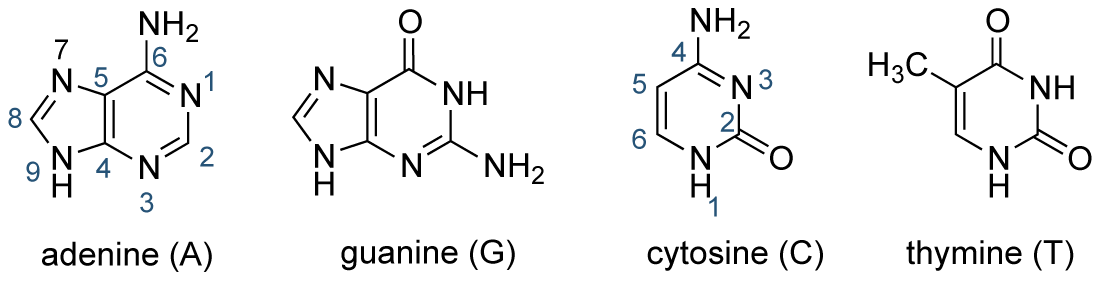
\includegraphics[scale=1.3]{DNA-heterocyclic-bases-large.png}
\end{center}
\caption{The four different nucleobases found in the DNA nucleotides~\cite{DNA-biotechacademy}.}
\end{figure}

The order of these nucleobases is what decides what function is encoded in any specific strand of DNA. A sequence of these nucleobases (a DNA sequence) can be called a genetic blueprint for proteins. During the production of proteins, a DNA sequence is either copied, or transcribed into ribonucleic acid (RNA). RNA decides which amino acids will be put together, which creates a corresponding protein.

RNA differentiates itself from DNA, among other things, by using uracil (U) instead of thymine. However, uracil and thymine are generally considered synonymous, as both bases binds with adenine. A DNA strand can bond with another DNA strand containing the complementary nucleobases.

\begin{definition}
\textbf{Complementarity} is defined as a nucleobase capable of bonding with another nucleobase.
\begin{center}
\begin{tabular}{|c|c|}
\hline
Base & Complementary base \\
\hline
G & C \\
T/U & A \\
C & G \\
A & T/U \\
\hline
\end{tabular}
\end{center}
\end{definition}

\begin{figure}[H]
	\label{Complementarity}
	\begin{center}
		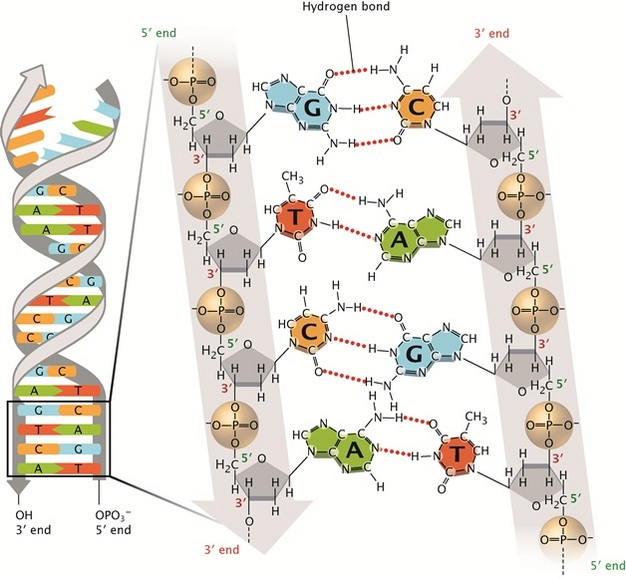
\includegraphics[scale=2.5]{complementarity.jpg}	
	\end{center}
	\caption{Hydrogen bonds between the nucleobases, which makes up the basis for complementarity~\cite{DNA-nature}.}
\end{figure}

Sometimes, you may wish to express a DNA sequence's complementary DNA sequence. This is called the complement of a given DNA sequence. The reverse of a complement is called the \textbf{reverse complement}.

\begin{definition}
For a given DNA sequence s, \~{s} is the sequence that contains the complementary bases of s, in reverse order.
\end{definition}

\subsection{Regular Expressions}

In order to talk about regular expressions, we need to be able to talk in general terms of languages. We can define a language as a subset of the infinite set of words or symbols, chosen from a finite alphabet. An alphabet with the letters $\{a,b\}$ might for example form the words $ab$, $ba$, $aab$ or any such combination of any length, thus forming an infinite set of words.\\

\begin{definition} An alphabet $\Sigma$ is defined as a finite non-empty set of characters.

\end{definition}

\begin{definition} Given an alphabet $\Sigma$, the language $\mathcal{A}$ is defined by $\mathcal{A} \subseteq \Sigma^*$, where $\Sigma^*$ is the set of all words constructed from alphabet $\Sigma$.
	
\end{definition} 

\begin{definition} Given an alphabet $\Sigma$, we define a grammar for a regular expression $E$.\\

	\begin{enumerate}
		\item An expression containing a single letter $a$ from our alphabet $\Sigma$: $E = a$. 
		\item The expression $E = 1$
		\item The expressions $E = 0$.
		\item A combination of two regular expressions $E_1$ and $E_2$:
		\begin{eqnarray}
			E &=& E_1 | E_2 \\
			E &=& E_1E_2 \\
			E &=& E_1^*
		\end{eqnarray}
	\end{enumerate}	
\end{definition} 

We can interpret the regular expression $E$ over the alphabet $\Sigma$ as a language denoted by $\mathcal{L}(E)$: \\

\begin{definition} The language $\mathcal{L}(E) \subseteq \Sigma^*$ for the regular expression $E$ from the alphabet $\Sigma$, is defined as.

	\begin{enumerate}
		\item For single-letter expressions we have
			\begin{eqnarray}
				\mathcal{L}(0) &=& \emptyset \\
				\mathcal{L}(1) &=& \{\epsilon\} \\
				\mathcal{L}(a) &=& \{a\}
			\end{eqnarray}
			Where $a \in \Sigma$
			
		\item For combined expressions we have
			\begin{eqnarray}
				\mathcal{L}(E_1|E_2) &=& \mathcal{L}(E_1) \cup \mathcal{L}(E_2) \\
				\mathcal{L}(E_1E_2) &=& \mathcal{L}(E_1) \odot \mathcal{L}(E_2) \\
				\mathcal{L}(E^*) &=& \bigcup^{\infty}_{n = 0}\mathcal{L}(E^n)
			\end{eqnarray}
			Where $\mathcal{L}(E_1) \odot \mathcal{L}(E_2) = \{w_1w_2 \ |\  w_1 \in \mathcal{L}(E_1), w_2 \in \mathcal{L}(E_2)\}$, and where \\
			$E^0 = 1, \ E^{n+1} = EE^n$.
	\end{enumerate}
\end{definition}


\subsubsection{Implementing regular expressions}

Now that we have defined regular expressions formally, we want to be able to match strings against them. We say that a regular expression $E$ matches a string $S$ if $S \in \mathcal{L}(E)$.
The industry standard way of solving this problem which regular expression implementations such as Google's RE2 use~\cite{matching-in-the-wild}, is through expressing the regular expression as a \textit{deterministic finite automata} (DFA) or a \textit{non-deterministic finite automata} (NFA) in accordance with Kleene's theorem~\cite{kleenes-theorem}. 

\begin{definition} A deterministic finite automaton is a five-tuple $(Q,\ \Sigma,\ \delta,\ q_0,\ F)$ where
\label{dfa definition}

\begin{itemize}
	\item $Q$ is a finite set of states
	\item $\Sigma$ is an alphabet
	\item $\delta$ is a transition function $\delta: Q \times \Sigma \rightarrow Q$
	\item $q_0$ is an initial state $q_0 \in Q$.
	\item $F$ is a set of accepting states $F \subseteq Q$.
\end{itemize}
\end{definition}

We define $q_i \xrightarrow{\gamma} q_j$ as the transition $(q_i, \gamma, q_j) \in \delta$ from $q_i$ to $q_j$ over edge $\gamma$ and we define $q_i \overset{\gamma}{\leadsto} q_j$ as $q_i \xrightarrow{\gamma_i} q_2 \xrightarrow{\gamma_{i+1}} ... \xrightarrow{\gamma_{j-1}} q_{j}$.
 
A DFA and an NFA can be illustrated as a graph where each vertex represents a state and each edge represents a transition. An example of a DFA can be seen in Figure~\ref{dfa_simple}. \\

\begin{figure}[H]
  \begin{center}

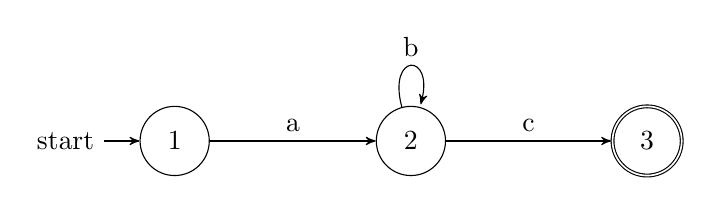
\begin{tikzpicture}[>=stealth', auto, node distance=3cm]
  \node[initial,state] (1) {$1$};
  \node[state] (2) [right of=1] {$2$};
  \node[state,accepting] (3) [right of=2] {$3$};
  
  \path[->] (1) edge node {a} (2);
  %\path[->] (2) edge [bend right] node {c} (3);
  \path[->] (2) edge [loop above] node {b} (3);
  \path[->] (2) edge node {c} (3);
\end{tikzpicture}
	
	\caption{DFA $Q = \{1, 2, 3\}$ matching the regular expression \underline{$ab*c$}}
	\label{dfa_simple}
  \end{center}
\end{figure}


\begin{definition} A non-deterministic finite automaton is a five-tuple $(Q,\ \Sigma,\ \delta,\ q_0,\ F)$ where

\begin{itemize}
	\item $Q$ is a finite set of states
	\item $\Sigma$ is an alphabet
	\item $\Delta$ is a transition function $\Delta \subseteq Q \times (\Sigma \cup \{\epsilon\}) \times Q$
	\item $q_0$ is an initial state $q_0 \in Q$.
	\item $F$ is a set of accepting states $F \subseteq Q$.
\end{itemize}

\label{nfa definition}
\end{definition}

We define $q \xrightarrow{\gamma} q'$ as the transition from $q$ to $q'$ over edge $\gamma$ also denoted $(q, \gamma, q') \in \Delta$, and we define $q \overset{\gamma}{\leadsto} q'$ as the transitions $q_1 \xrightarrow{\gamma_1} q_{2} \xrightarrow{\gamma_{2}} ... \xrightarrow{\gamma_{n}} q_{n+1}$.

While a state $q_i$ in a DFA has only one possible transition candicate $q_j$, an NFA simulation needs to evaluate all possible transition candidates until it reaches their final state. If any of the final states is in the set of accepting states $F$, the NFA matches the input string.

\begin{figure}[H]
  \begin{center}

\begin{tikzpicture}[>=stealth', node distance=3cm]
  \node[initial,state] (1) {$1$};
  \node[state] (2) [right of=1] {$2$};
  \node[state] (3) [above of=2] {$3$};
  \node[state] (4) [below of=2] {$4$};
  \node[state,accepting] (5) [right of=2] {$5$};
  
  \tikzset{edge_label/.style={->}} 
  \tikzset{every node/.style={fill=white}} 
  
  \path[->] (1) edge [edge_label] node {a} (2);
  \path[->] (1) edge [edge_label] node {a} (3);
  \path[->] (1) edge [edge_label] node {a} (4);
  \path[->] (2) edge [edge_label] node {b} (5);
  \path[->] (3) edge [edge_label] node {c} (5);
  \path[->] (4) edge [edge_label] node {d} (5);
\end{tikzpicture}
	
	\caption{NFA $Q = \{1, 2, 3, 4, 5\}$ matching the regular expression \underline{$ab|c|d$}}
	\label{nfa_simple}
  \end{center}
\end{figure}

In Figure~\ref{nfa_simple} we see how an NFA simulation must choose between multiple transition candidates upon finding an $a$ in our input sequence, and thus have to try all of them concurrently in order to try to reach the accepting state. It is worth noting that any DFA can be constructed from an NFA but at the cost of exponential blow-up in number of states and memory consumption~\cite{nfa-to-dfa}.

An NFA can be simulated in the following simple manner where the NFA accepts string $s$ if $q_0 \in Reach(Close(F), s)$.
\begin{eqnarray}
	Reach(M, \epsilon) & = & M \\
	Reach(M, ab) & = & Reach(Reach(M, a), b) \\
	Reach(M, a) & = & \epsilon-Closure(Step(M, a)) \\
	Step(M, a) & = & \{ q'\ |\ q \in M, q \xrightarrow{a} q' \} \\
	\epsilon-Closure(M) & = & \{ q'\ |\ q \in M, q \overset{\epsilon}{\leadsto} q' \}
\end{eqnarray}

An example of this simulation is shown in Example~\ref{example:nfa_epsilon_example}.

\begin{figure}[H]
  \begin{center}

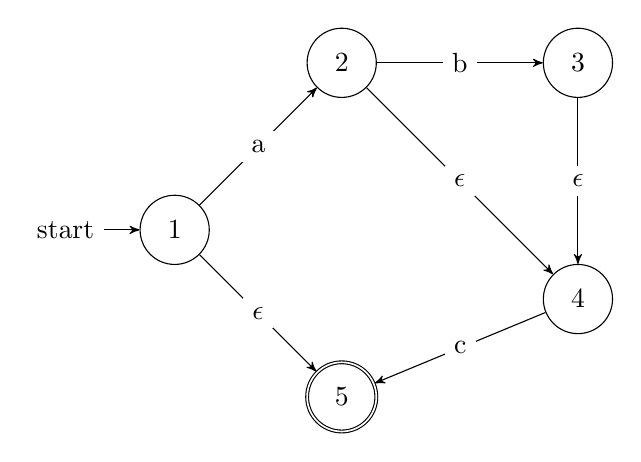
\begin{tikzpicture}[>=stealth', node distance=3cm]
  \node[initial,state] (1) {$1$};
  \node[state] (2) [above right of=1] {$2$};
  \node[state] (3) [right of=2] {$3$};
  \node[state] (4) [below of=3] {$4$};
  \node[state,accepting] (5) [below right of=1] {$5$};
  
  \tikzset{edge_label/.style={->}} 
  \tikzset{every node/.style={fill=white}} 
  
  \path[->] (1) edge [edge_label] node {a} (2);
  \path[->] (1) edge [edge_label] node {$\epsilon$} (5);
  \path[->] (2) edge [edge_label] node {b} (3);
  \path[->] (2) edge [edge_label] node {$\epsilon$} (4);
  \path[->] (3) edge [edge_label] node {$\epsilon$} (4);
  \path[->] (4) edge [edge_label] node {c} (5);
\end{tikzpicture}
	
	\caption{NFA $Q = \{1, 2, 3, 4, 5\}$ matching the regular expression \underline{$(ab?c)?$}}
	\label{nfa_epsilon}
  \end{center}
\end{figure}

\begin{example}
\label{example:nfa_epsilon_example}
Simulating NFA in Figure \ref{nfa_epsilon}, where $Q = \{1, 2, 3, 4, 5\}$, $q_0 = 1$ and $F = 5$ and the input string $abc$. \\


\end{example}

\section{Patscan as regular expressions}

The most notable of the SFM format's features, is the possibility to search for \textit{mismatches}, \textit{insertions} and \textit{deletions} in a given or stored sequence. 

\begin{definition}
	The number of \textbf{mismatches} in a sequence, is the number of random characters in the sequence which may be switched with any other character from the alphabet.
\end{definition}

\begin{definition}
	The number of \textbf{insertions} in a sequence, is the number of additional characters from the alphabet which may be inserted anywhere in the sequence.
\end{definition}

\begin{definition}
	The number of \textbf{deletions} in a sequence, is the number of random characters in the sequence which may be deleted.
\end{definition}

The sequence \texttt{AGTCT} can be extended to \texttt{AGTCT[1,1,1]} in order to match up to one mismatch, up to one insertion, up to one deletion or any combination thereof. This means that a sequence of length $n$ with a single mismatch will yield $n^1+1$ possible matches of the data string. \texttt{AGTCT[1,0,0]} will for instance match any of the following, where \_ represents a mismatch.

\texttt{AGTCT, \_GTCT, A\_TCT, AG\_CT, AGT\_T, AGTC\_}

Another powerful feature of patscan is the ability to store a sub-pattern match in a named variable. If a match is found for the named variable in the beginning of a pattern for instance, this match can then be referenced later in the same pattern, by using the variable name. An example of this could be the pattern \texttt{p1=2...4 10...20 {\raise.17ex\hbox{$\scriptstyle\mathtt{\sim}$}}p1}. This pattern will match the contents of \texttt{p1}, followed by any 10 to 20 characters, followed by the match stored in \texttt{p1}, but with the reverse complement as denoted by the \texttt{{\raise.17ex\hbox{$\scriptstyle\mathtt{\sim}$}}}. This is similar to the back-referencing functionality for capturing groups, which many popular regular expression implementations support.%\cite{indsæt citation her.}

This 'combination' notation as well as the ability to store sequences in variables and matching them further down the pattern, makes the patscan language very compact compared to regular expressions. A pattern as simple as \texttt{p1=8...16 10...50 ~p1[2,0,1]} describes a complex relationship, which cannot easily be discovered through REs.

\subsection{Grammar}
\label{Patscan grammar}

SFM uses an alphabet, which is the set of characters allowed in a patscan sequence. This set is from the nucleobases, that is found in DNA and RNA. While we have chosen not touch upon this subject, it is worth noting that SFM can also be used for matching in protein sequences.
\begin{definition}
The alphabet, that makes up DNA sequences, denoted by $\mathcal{A}_{DNA}$ is:
\begin{center}
$\mathcal{A}_{DNA}$ = \texttt{\{A, T, C, G\}}
\end{center}
\end{definition}

\begin{definition}
The alphabet, that makes up RNA sequences, denoted by $\mathcal{A}_{RNA}$ is:
\begin{center}
$\mathcal{A}_{RNA}$ = \texttt{\{A, U, C, G\}}
\end{center}
\end{definition}

Besides the five basic nucleobases in $\mathcal{A}_{DNA} \cup \mathcal{A}_{RNA}$, 11 ambiguity characters also exist~\cite{DNA-sciencedaily}. These ambiguity characters were designed for positional variations in families of related genes. The ambiguity characters are named so because they represent an uncertainty in the sequencing program of which nucleobases is actually at that spot~\cite{ambiguitycodes, dna-base-error-rate}.

\begin{definition}
The alphabet, that makes up DNA and RNA sequences, as well as the ambiguity characters, denoted by $\mathcal{A}$ is:
\begin{center}
$\mathcal{A}$ = \texttt{\{A, T, U, G, C, Y, R, S, W, K, M, B, D, H, V, N\}}
\end{center}
\end{definition}

The patscan language has the following grammar, where char is any character from the alphabet $\mathcal{A}$.

\begin{figure}[H]
\begin{center}
\begin{tabular}{|lcll|}
	\hline
	$Prog$ &  $\rightarrow$ & list of $Stmt$ & \\
	$Stmt$ & $\rightarrow$ & $Exp$ & \\
	\enspace & $|$ & $LVal1\ =\ Exp$ &  \textcolor{red}{Variable assignment} \\
	\enspace & $|$ & $LVal2$ & \textcolor{red}{Variable usage} \\
	$LVal1$ & $\rightarrow$ & \textbf{Id} & \textcolor{red}{Ids may not be reassigned}\\
	$LVal2$ & $\rightarrow$ & \textbf{Id} $Combi$ & \\
	\enspace & $|$ & {\raise.17ex\hbox{$\scriptstyle\mathtt{\sim}$}} \textbf{Id} $Combi$ & \\
	$Exp$ & $\rightarrow$ & \textbf{num} ... \textbf{num} & \textcolor{red}{Range} \\
	\enspace & $|$ & $Seq\ Combi$ & \\
	$Seq$ & $\rightarrow$ & list of \textbf{char} & \\
	$Combi$ & $\rightarrow$ & [\textbf{num},\textbf{num},\textbf{num}] & \\
	\enspace & $|$ & $\epsilon$ & \\
	\hline
\end{tabular}
\end{center}
\caption{PatScan grammar}
\end{figure}

The patscan language can be broken down into a few simple components or tokens, which we will refer to as sub-patterns. We have divided the sub-patterns into the following classes:

The sub-patterns which consist only of a consecutive sequence of characters from $\mathcal{A}$, is denoted as a \textbf{sequence} (Example: \texttt{AGTCT})

The sub-patterns which consist of a consecutive sequence of characters from $\mathcal{A}$, followed by square brackets, containing three numbers (each representing \textbf{mismatches}, \textbf{deletions}, and \textbf{insertions} respectively), is denoted as a \textbf{combination sequence} (Example: \texttt{AGTCT[1,0,0]})

The sub-patterns which consist of a number, $a \geq 0$, followed by exactly three dots, followed by a number, $b \geq a$, is denoted as a \textbf{range} (Example: \texttt{2...4})

The sub-patterns which consist of a string, denoted as a \textbf{variable name}, followed by an equal sign, and then a \textbf{sequence}, is denoted as a \textbf{variable assignment} (Example: \texttt{p1=AGTCT})

The sub-patterns which consist only of a \textbf{variable name}, is denoted as a \textbf{variable usage} (Example: \texttt{p1})

The reverse complement of a sequence or variable is denoted by placing a \texttt{{\raise.17ex\hbox{$\scriptstyle\mathtt{\sim}$}}} directly in front of the sequence or variable.

\subsection{Ranges}

Patscan ranges are very similar to RE ranges, and is therefore easily translated. A patscan range, which has the form:
\begin{equation}
\label{example:range}
	2...5
\end{equation}
Translates into 'from 2 to 5 of any character'. In the general syntax of RE, there is a character for 'any character', which is \texttt{.} and a quantifier which enables you to state how many of a given character or group you want matched, which is \texttt{\{min,max\}}. Using these, (\ref{example:range}) translates into the following RE:
\begin{equation}
.\{2,5\}
\end{equation}

\subsection{Mismatches, Deletions, and Insertions}

Combination sequences do not exist in REs. One way to represent these sub-patterns as REs is by constructing every possible combination of the sequence defined by the patscan notation.

A recursive algorithm $f$ that solves this problem can easily be written, but it will have an exponential running time in the length of the sequence. 

\begin{example}[label=example:recursion]
Looking at the combination sequence \texttt{AGCTC[2,0,0]}, we start by taking the \texttt{A}, and call $f$ with the remaining letters for every possibility of the \texttt{A}.
\begin{eqnarray}
	Left\ branch &=& f(\texttt{A}, \texttt{GCTC[2,0,0]}) \\
	right\ branch &=& f(mismatch(\texttt{A}), \texttt{GCTC[1,0,0]})
\end{eqnarray}
The left branch will continue recursively with \texttt{GCTC[2,0,0]}, and the right branch will do the same but with only one mismatch available, since we already chose \texttt{A} as our first mismatch. When $f$ reaches its base case, we will have a string with a unique combination of mismatches. All possible combinations can be constructed with this approach.
\end{example}

Adding deletions and insertions to \textbf{example \ref{example:recursion}} will increase the number of possibilities for each letter thus increasing the recursion depth. The recursion does not bottom out until every combination is found. This means that if the sequence is large enough (This can happen already at a length of 20, if not earlier, depending on the number of mismatches, insertions, and deletions), the program will reach maximum recursion depth (depending on the programming language), or run out of memory before terminating.

In order to guarantee a low recursion depth, we use a divide and conquer Algorithm~\cite{Algorithms}, which reduces the recursion depth to $log(n)$. This works by splitting the sequence in two halves per recursion, such that at the deepest recursion level, we have sequences of only a single character, as can be seen in Figure \ref{fig:tree_example}. 

\begin{figure}[H]
\begin{tikzpicture}[->,>=stealth',level/.style={sibling distance = 5cm/#1,
  level distance = 1.5cm}] 
\node [arn_n] {abcd}
	child{ node [arn_n] {ab} 
		child{ node [arn_n] {a}}
		child{ node [arn_n] {b}}                            
	}
    child{ node [arn_n] {cd}
		child{ node [arn_n] {c}}
		child{ node [arn_n] {d}}
	}
; 
\end{tikzpicture}
	\centering
	\caption{Tree structure, showing the steps taken by the algorithm during the divide step.}
	\label{fig:tree_example}
\end{figure}

After dividing the sequence into characters and reaching the \emph{base case}, we have to 'conquer' each sub-problem. On the lowest recursion level (where the sequence is a single character), Algorithm~\ref{alg:divideandconquer} will make a list of all possibilities for that character.

\begin{definition}[label=definition:possibilities]
When reaching base case for a character $a$, Algorithm~\ref{alg:divideandconquer} will construct the following possibilities for mismatches and deletions

\begin{center}
	\texttt{a, \^{}a, \_}
\end{center}

\noindent as well as the following for insertions

\begin{center}
	\texttt{.\{1\}a, .\{2\}a, $\cdots$, .\{n\}a} \\
	\texttt{a.\{1\}, a.\{2\}, $\cdots$, a.\{n\}}
\end{center}

\noindent This list of possibilities for $a$ defines that $a$ may take the form of a mismatch (\texttt{\^{}a}), its original form, or any of the other forms in the list. The list of possibilities is then returned and can be combined with the list received from the 'b' recursion.
\end{definition}

\emph{Combining} two such lists means that each element in the left list is concatenated behind each element in the right list. As such, a new list of size $m \times n$ will be created. The total number of mismatches, deletions, and insertions are being kept track of, and if a combination of two elements will result in more mismatches, deletions, or insertions than the maximum allowed, it is skipped.

\subsection{Algorithm}

\begin{spacing}{0.8}
\begin{algorithm}[H]
	\caption{find\_combinations}
	\label{alg:divideandconquer}
  	\begin{algorithmic}[1]
    		\Require
    			\Statex $seq$ - sequence string to be translated
    			\Statex $m_{max}$ - allowed number of mismatches
    			\Statex $d_{max}$ - allowed number of deletions
    			\Statex $i_{max}$ - allowed number of insertions
    		\Ensure
    			\Statex List of all possible combinations
		\Statex
		\Function{find\_combinations}{$seq$, $m_{max}$, $d_{max}$, $i_{max}$}
    		\If{$seq.length > 1$}
    			\Let{left\_tree}{\Call{find\_combinations}{seq[0..(seq.length/2).floor-1], $m_{max}$, $i_{max}$, $d_{max}$}} \label{alg:divide:leftT}
    			\Let{right\_tree}{\Call{find\_combinations}{seq[(seq.length/2).floor..-1], $m_{max}$, $i_{max}$, $d_{max}$}} \label{alg:divide:rightT}
    		\Else
    			\Returns{List of all mismatch, insertion, and deletion combinations of seq} \label{alg:divide:conquer}
    		\EndIf
    		\State
    		\Let{combined}{empty list}
    		\Let{unique\_combinations}{empty set}
    		\ForAll{LL \In left\_tree} \Comment{LL: Left leaf}
    			\ForAll{RL \textbf{in} right\_tree} \label{alg:divide:inner} \Comment{RL: Right leaf}
    				\If{$LL.m + RL.m > m_{max}$ \Or $LL.d + RL.d > d_{max}$ \Or $LL.i + RL.i > i_{max}$} \label{alg:divide:invariant1}
    					\State continue
    				\EndIf
    				\If{\Not LL.seq + RL.seq \In unique\_combinations.keys} \label{alg:divide:invariant2}
    					\Let{unique\_combinations}{LL.seq + RL.seq}
    					\Let{combined}{LL + RL}
    				\EndIf
    			\EndFor
    		\EndFor
    		\Returns{combined}
    		\EndFunction
  	\end{algorithmic}
\end{algorithm}
\end{spacing}


\subsubsection{Correctness}

We wish to show that Algorithm~\ref{alg:divideandconquer} is correct, by showing that given a set of parameters which meets a pre-condition, Algorithm~\ref{alg:divideandconquer} will arrive at a result which satisfies a post-condition. Additionally we must also make sure that Algorithm~\ref{alg:divideandconquer} satisfies an invariant in all iterations.

Pre-conditions:
\begin{itemize}
\item[-] seq is a string of length $i > 0$
\item[-] $m_{max}$ is a non-negative integer
\item[-] $d_{max}$ is a non-negative integer
\item[-] $i_{max}$ is a non-negative integer
\end{itemize}

Post-condition:
\begin{itemize}
\item[-] The list $combined$ contains all combinations of the initial sequence with up to  $m_{max}$ mismatches, $d_{max}$ deletions, and $i_{max}$ insertions.
\end{itemize}


We start by showing the correctness of the inner loop. For this we have the following loop invariant which must be satisfied during all iterations of the loop.

\textbf{For a given element $a$, and another element $B[j]$, a combination of the two yields a new unique element $c$, such that $c_m \leq m_{max}$, $c_d \leq d_{max}$, $c_i \leq i_{max}$, where $c_m$, $c_d$, $c_i$ is the number of $c$'s mismatches, deletions and insertions respectively.}

\begin{itemize}
\item Initialization:
\begin{itemize}
	\item[] Prior to the loop at line~\ref{alg:divide:inner}, the invariant is respected (trivially), as $B[j]$ is \textbf{null}.
\end{itemize}

\item Maintenance:
\begin{itemize}
	\item[] For $j = k$, the loop will have an element $a$ (\texttt{LL}), and an element $B[j]$ (RL), which both respect the condition of the invariant. Before combining $a$ and $B[j]$, the condition of the invariant is checked at line~\ref{alg:divide:invariant1} and line~\ref{alg:divide:invariant2}. If the invariant is not satisfied, the combining of $a$ and $B[j]$ is skipped.
\end{itemize}

\item Termination:
\begin{itemize}
	\item[] When the loop terminates, the invariant will be true on the output.
\end{itemize}
\end{itemize}

Since the invariant is satisfied for the inner loop, the same can be concluded for the outer loop as it iterates over iterations of the inner loop. The invariant for the outer loop can be seen as multiple of the inner loop's invariant.

Next, we wish to show that the recursion is correct. For this we have the invariant $I(n)$:

\textbf{For a set $A$, and a set $B$, a combination of the two where each element in $A$ is combined with each element in $B$ separately yields a set $C$, such that all $e \in C$ satisfies $e_m \leq m_{max}$, $e_d \leq d_{max}$, $e_i \leq i_{max}$, where $e_m$, $e_d$, $e_i$ is the number of $e$'s mismatches, deletions and insertions respectively.}


\begin{itemize}
\item Initialization:
\begin{itemize}
	\item[] Prior to the recursion step at line~\ref{alg:divide:leftT} and line~\ref{alg:divide:rightT}, the invariant is respected (trivially), as set $A$ and $B$ are empty..
\end{itemize}

\item Maintenance:
\begin{itemize}
	\item[] For combining at step $k$, the algorithm will have two sets of valid elements (respects the condition of the invariant), from which it will construct a new set of all combinations of the elements in the two original sets. This combination follows the invariant of the inner loop, and will thus also respect the recursion invariant.
\end{itemize}

\item Termination:
\begin{itemize}
	\item[] When the recursion terminates, the invariant will be true on the entire output.
\end{itemize}
\end{itemize}


\subsubsection{Redundancy}

Using Algorithm~\ref{alg:divideandconquer} without modifications will cause a lot of redundancy when translating insertions. This comes from the fact that we wish to construct all possible combinations recursively.

If we look at the combination sequence \texttt{ab[0,0,1]}, the possible outcomes of \texttt{a} (at the lowest level of recursion) can be \texttt{a}, \texttt{.a}, and \texttt{a.}, and the same for \texttt{b}. Combining these, we will have two different cases of \texttt{a.b} (\texttt{a. b} and \texttt{a .b}). It is redundant to keep both and doing so will create exponentially more redundancy growing with recursion depth.

Assuming we have an even number of characters in the sequence and that only insertions are allowed, we have that on the first 'combine' step there are
\begin{eqnarray}
	\label{r_0}
	r_0 = \frac{1}{2}n\sum^{i_{max}}_{i=1} i
\end{eqnarray}

redundant cases, where $\frac{1}{2}n$ is the number of combine steps on this recursion level.

\begin{example}
The following example shows the variations of $a$ with $b$ which are the same when combined. The bold characters are combined with the cursive characters.
\begin{eqnarray}
	i_{1}: \textbf{a.}b\ \ \textbf{a}.b = 2 - 1 = 1 \\
	i_{2}: \textbf{a..}b\ \ \textbf{a.}.b\ \ \textbf{a}..b = 3 - 1 = 2 \\
	i_{3}: \textbf{a...}b\ \ \textbf{a..}.b\ \ \textbf{a.}..b\ \ \textbf{a}...b = 4 - 1 = 3
\end{eqnarray}
For $i_{1}$ we have 2 cases which are the same. One of these is redundant giving us $2 - 1 = 1$ redundant cases. \\
Since all cases for $i_{n-1}$ also applies to $i_{n}$, we end up with
\begin{eqnarray}
	\sum_{i=1}^{i_{max}}i
\end{eqnarray}
redundant cases for each combination step in each branch, where $i_{max}$ is the maximum number of insertions. If $n$ is the number of characters in the sequence, there are $\frac{1}{2}n$ combination steps on this level, which gives us:
\begin{eqnarray}
	r_0 = \frac{1}{2}n\sum^{i_{max}}_{i=1} i
\end{eqnarray}
\end{example}

On the next combine step we have $r_1$ redundant cases. In order to calculate $r_1$ we will define $c = 1 + 2i$ as the number of cases in the \textit{base case}, meaning the number of cases on the lowest level of the recursion. Each redundant case will be combined with all cases in the second set, which contains $c^2$ cases. All non-redundant cases from the first set will also be combined with all redundant cases of the second set. 

A lot of combinations will be skipped because there is a varying maximum number of insertions allowed in a single case, resulting in fewer cases than $c^2$. To correct for this we will introduce a factor $\kappa$ which represents the scaling factor.
\begin{eqnarray}
	\label{r_1}
	r_1 = \frac{1}{4}n(2r_0\frac{c^2}{\kappa_1} - r_0^2)
\end{eqnarray}

\begin{example}
We have a set $A$ and another set $B$, each containing $\frac{c^2}{\kappa}$ elements, of which $r_0$ are redundant.

All $r_0$ redundant elements in $A$ will combine with all elements in $B$, creating $r_0\frac{c^2}{\kappa}$ redundant cases. Likewise, all $\frac{c^2}{\kappa}-r_0$ non-redundant cases in $A$ will combine with all $r_0$ redundant cases in $B$, creating $r_0(\frac{c^2}{\kappa}-r_0)$ additional redundant cases. There are $\frac{1}{4}n$ combination steps on this level, which gives us:
\begin{eqnarray}
	r_1 &=& \frac{1}{4}n(r_0\frac{c^2}{\kappa_1} + r_0(\frac{c^2}{\kappa_1} - r_0))\\
		&=& \frac{1}{4}n(r_0\frac{c^2}{\kappa_1} + r_0\frac{c^2}{\kappa_1} - r_0^2))\\
		&=& \frac{1}{4}n(2r_0\frac{c^2}{\kappa_1} - r_0^2)
\end{eqnarray}
\end{example}

We can then calculate the total amount of redundancy of any sequence with $logn$ recursion depth, via induction:
\begin{eqnarray}
	r_x &=& \frac{1}{2^{x+1}}n (r_{x-1}\frac{c^{2^{x+1}}}{\kappa_x} + r_{x-1}(\frac{c^{2^{x+1}}}{\kappa_x} - r_{x-1}))\\
		&=& \frac{1}{2^{x+1}}n (r_{x-1}\frac{c^{2^{x+1}}}{\kappa_x} + r_{x-1}\frac{c^{2^{x+1}}}{\kappa_x} - r_{x-1}^2)\\
		\label{r_x}
		&=& \frac{1}{2^{x+1}}n (2r_{x-1}\frac{c^{2^{x+1}}}{\kappa_x} - r_{x-1}^{2^{x+1}})
\end{eqnarray}

Here $x$ is the recursion dept, and will thus go up to $logn$, where $n$ is the length of the patscan sequence.

Given a pattern where mismatches and deletions are allowed as well as insertions, the amount of redundancy increases, as $c$ will grow larger.

Despite the result reached in (\ref{r_x}), inaccuracy occurs as the recursion depth varies in the recursion branches based on the length of the original string, as shown in Figure~\ref{fig:recursion_depth_example}.

\begin{figure}[H]
\begin{tikzpicture}[->,>=stealth',level/.style={sibling distance = 5cm/#1,
  level distance = 1.5cm}] 
\node [arn_n] {abc}
	child{ node [arn_n] {a}}
    child{ node [arn_n] {bc}
		child{ node [arn_n] {b}}
		child{ node [arn_n] {c}}
	}
; 
\end{tikzpicture}
	\centering
	\caption{Tree structure showing how recursion depth varies in different branches.}
	\label{fig:recursion_depth_example}
\end{figure}

Despite of this inaccuracy it is obvious that removing the redundancy would translate into better running times.

Avoiding this redundancy is very important and relatively trivial. Every time two cases are combined, the new combination is put in a set data structure, which we use to check future combinations. If a future combination already exists in the set, it is skipped thus avoiding duplicates. By avoiding duplicates early on in Algorithm~\ref{alg:divideandconquer}, we save a lot of memory and running time for both the translation of the regular expressions and of the regular expressions themselves.

\subsubsection{Running time}

In the divide step, Algorithm~\ref{alg:divideandconquer} first splits a given sequence in half multiple times until it reaches base case (where length of the sequence is one). It does this recursively with a branching factor of two, and splitting takes constant time, meaning the running time so far is 
\begin{eqnarray}
	T(n) = 2T(\frac{n}{2}) + O(1) = O(n)
\end{eqnarray}

The conquer step where we construct each combination of every base case, is trivially solved by constructing a set of the combinations. We construct one element if any mismatches are allowed, which we can do in $O(1)$ constant time. We construct one element if any deletions are allowed, which we can also do in $O(1)$ constant time. We construct two elements for each insertions that is allowed, which take $O(2i)$ time where $i$ is the number of insertions allowed. It does this for every base case, which leaves us with a total running time of $O(ni)$.
\begin{eqnarray}
	T(n) = O(n) + O(ni)
\end{eqnarray}

In the combine step we combine each element of two sets $A$ and $B$. Each combination takes $O(1)$ constant time, and we perform this operation $|A| \cdot |B|$ times. The sets $A$ and $B$ were created in the same way recursively, which means that the total running time of each recursion level increases exponentially. In total we have a running time of $O(i^n)$, where $i$ is the number of insertions, and $n$ is the length of the sequence.

The running time of every combination step before the final one combined is significantly smaller than the final combination step, which means that they are consumed by the exponentially larger running time of the last iteration. This gives us a running time of:
\begin{eqnarray}
	T(n) = O(n) + O(ni) + O(i^n)
\end{eqnarray}

The running time of the divide and conquer step is also consumed by the combine step leaving us with a running time of
\begin{eqnarray}
	O(i^n)
\end{eqnarray}

\subsection{Variable assignments \& usage}

Variable assignment is when you assign a pattern to a variable in order to reuse the pattern. Any kind of non-variable pattern may be used in a variable pattern. Hence we have three different kinds of variable assignments:

\texttt{p1=ATCG} \\
\texttt{p2=ATCG[2,0,0]} \\
\texttt{p3=2...4}

These assignments can be referenced by using the variable name. An example of such usage could be

\texttt{p4=ACCT 2...5 p4}

In addition to referencing the variable, a variable may also be inverted. This is denoted by using a tilde character prepended onto the variable:

\texttt{{\raise.17ex\hbox{$\scriptstyle\mathtt{\sim}$}}p4}

Here, inversion refers to the reverse complement of the sequence stored in the variable.

Sequence and combination assignments are implemented by translating the sequence or combination and storing the translated regular expression in a table with the variable name as the key. If the variable is then later used in the patscan pattern, the translated sequence or combination may be placed into the full regular expression. This way there are no actual back-references in the regular expression.

Assignment of a range is something we have chosen not to implement, as it can't be implemented without the use of back-referencing, because there is no way of knowing what the contents of a range will actually be.

\section{Experiment}

The following experiment was conducted in Ubuntu 14.04LTS, running a Intel i7-4558U Processor, 8Gb of DDR3L 1600 MHz SDRAM and two 256Gb SanDisk SD6SP1M256G1002 490MB/s read 350MB/s write solid state drives.

\subsection{RE Implementation Details}

In order to test regular expressions against different regular expression implementations, we created a small series of wrapper programs which take a regular expression and a text file to search as arguments and performs the matching and outputs the match results.

\subsubsection{Ruby}

The Ruby regular expression implementation uses an open source regular expression library called Oniguruma~\cite{oniguruma} which has support for multi-byte characters. The Oniguruma library creates a set of instructions for Oniguruma's virtual machine which performs the actual matching. This implementation can have an exponential running time for pathological regular expressions such as $(a?)^na^n$, since the Oniguruma's virtual machine uses a backtracking Algorithm~\cite{oniguruma-overview}.

Our wrapper program uses the built-in implementation in a straight-forward manner. Ruby does not support finding all matches at once, and thus we use the \texttt{scan} method to retrieve all results.

\begin{figure}[H]
	\begin{lstlisting}
	matches = fasta_file.to_enum(:scan, regex).map { Regexp.last_match }
	\end{lstlisting}
	\caption{Ruby for finding all matches of \texttt{regex} in \texttt{fasta\_file}.}
\end{figure}

\subsubsection{Python}

The Python regular expression implementation is based on PCRE~\cite{pcre}, but does vary in certain cases where the implementation will try to make some optimizations. The fact that the implementation is based on PCRE means that it can potentially have exponential running time~\cite{pcre-running-time}.

Python also does not allow the $(?i)$ and $(?-i)$ modifiers, and as such our wrapper program filters these out and instead adds the corresponding \texttt{IGNORECASE} flag.

\begin{figure}[H]
	\begin{lstlisting}
	results = re.findall(reg[4:-5], text, re.IGNORECASE)[0]
	\end{lstlisting}
	\caption{Python for finding all matches of \texttt{reg} in \texttt{text}, where it ignores lower/upper case.}
\end{figure}


\subsubsection{Python Regex}

The \mbox{\emph{Python}} Regex (PR) module is a regular expression implementation, that will eventually replace the current RE module. Similarly to its predecessor, PR is based on PCRE. While also trying to make some optimizations, PR do follow Perl and PCRE a bit more than the RE module.

Much like our wrapper for the standard python re module, we find all matches using PR like so:
\begin{figure}[H]
	\begin{lstlisting}
	p = regex.compile(reg[4:-6]);
	counter = len(p.findall(text, regex.IGNORECASE))
	\end{lstlisting}
	\caption{PR for finding all matches of \texttt{reg} in \texttt{text}, where it ignores lower/upper case.}
\end{figure}


\subsubsection{RE2}

Google's RE2 constructs DFAs or NFAs from the given regular expressions and thus guarantees linear running time~\cite{pcre-running-time}, but leaving behind support for back-references which are part of standard PCRE.

We have made small modifications to the RE2 library in order for it to support regular expressions of very large sizes, such as the ones we wish to run~\footnote{https://github.com/ttsoftware/re2}.

Our wrapper program for RE2 simply uses the built-in \texttt{FindAndConsume} method to find all the matches to the given regular expression.

\begin{figure}[H]
	\begin{lstlisting}
	FileService fr;
    string regexp = fr.read(argv[1]);
    string fasta = fr.read(argv[2]);

    RE2 pattern(regexp);

    StringPiece input(fasta);
    string value;
    
    int matches = 0;

    while (RE2::FindAndConsume(&input, pattern, &value)) {
        matches++;
    }
	\end{lstlisting}
	\caption{C++ which uses the RE2 library to find all matches of \texttt{pattern} in \texttt{input}}
\end{figure}

\subsection{Data Analysis}

We have chosen chromosome number 22 from the human genome, which is one of the smallest at approximately 50MB. Our version of chromosome 22 contains a lot of noise in the form of N's especially in the beginning of the file. These N's specify unknown bases during sequencing~\cite{human-genome}. We have decided not to modify the contents of the fasta file, since we want our tests to be close to a realistic usage scenario.

We could possibly have removed the N's and the linebreaks from the fasta file, in order to reduce the file size and thus reduce the runningtime of the regular expressions which we generate. However we felt that this would not significantly improve our results, and also make our test further from a real-world scenario.

\subsection{Experiment design}

We have set up a testing environment for our regular expressions, which consists of a series of patscan patterns. These patterns are grouped as mismatches, insertions, deletions, mixed combinations, ranges and sequences. Each group contains roughly 48 patscan pattern files with increasing complexity such that we test both simple and advanced patterns since the more advanced patterns translates into large regular expressions. 

\subsubsection{Mismatches, Deletions \& Insertions}
The mismatches, deletions and insertions patterns are further grouped into different series, where the first series range from a four-character sequence with one mismatch for instance, to a 16-character sequence with one mismatch. The second series is identical except each with two mismatches. We continue this way until we reach four mismatches, thus totalling at 48 different mismatch patterns.

\begin{example}
An example of a mismatch series.

\begin{center}
\texttt{AGCT[1,0,0], AGCTC[1,0,0], AGCTCT[1,0,0], ..., AGCTCTCCGTAACGGA[1,0,0]
AGCT[2,0,0], AGCTC[2,0,0], AGCTCT[2,0,0], ..., AGCTCTCCGTAACGGA[2,0,0]
}
\end{center}
\end{example}

\subsubsection{Mixed combinations}
The patterns with mixed combinations are grouped similarly to the mismatches, deletions and insertions patterns.

\begin{example}
An example of the different combination series.

\begin{center}
\texttt{AGCT[1,1,0], AGCTC[1,1,0], AGCTCT[1,1,0], ..., AGCTCTCCGTAACGGA[1,1,0]
AGCT[0,1,1], AGCTC[0,1,1], AGCTCT[0,1,1], ..., AGCTCTCCGTAACGGA[0,1,1]
AGCT[1,0,1], AGCTC[1,0,1], AGCTCT[1,0,1], ..., AGCTCTCCGTAACGGA[1,0,1]
AGCT[1,1,1], AGCTC[1,1,1], AGCTCT[1,1,1], ..., AGCTCTCCGTAACGGA[1,1,1]
}
\end{center}

\end{example}

\subsubsection{Ranges}

For the ranges patterns we have a single series where we increase the lower bound by two and the upper bound by four 47 times, thus generating a total of 48 patscan pattern files similarly to the other test groups. The length of the sequences on both side of the range stays the same for all the different range patterns.

\begin{example}
An example of the ranges series.

\begin{center}
\texttt{AGCTCT 2...4 AGCTCT, AGCTCT 4...8 AGCTCT, ..., AGCTCT 96...192 AGCTCT}
\end{center}
\end{example}

\subsubsection{Sequences}

For the sequence patterns we simply generate 48 patterns of different sizes. We start with a pattern of four characters and increment the number of characters by one until we reach 48.

\begin{example}
An example of the sequence series.

\begin{center}
\texttt{AGCT, AGCTC, AGCTCT, ..., AGCTCTCCGTAACGGAAGCTCTCCGTAACGGAAGCTCTCCGTAACGGA}
\end{center}
\end{example}

\subsubsection{Benchmarking the patterns}

We run each group against our chosen regular expression implementations which include Ruby, Python and our own version of Google's RE2.
 
Each pattern file is translated using our Ruby implementation of the algorithm described in Algorithm~\ref{alg:divideandconquer}. The resulting regular expressions is subsequently stored in a file and passed as an argument to the regular expression implementations. Each patscan file is benchmarked in its own thread in order to take advantage of our multicore / multithreaded testing computer. Each thread is also given a time limit of 1 minute after which the thread is killed. This time limit is given because the difference between taking 1 minutes and 2 minutes is insignificant compared to SFM' in-the-seconds running time, and thus the program might as well never finish.

The outputs of our wrapper programs are piped to a result file for each regular expression implementation and pattern.

\begin{example} 
An example of a result file.
\begin{verbatim}
PATSCAN: GGGCCC[0,1,0]
LENGTH OF RE: 35
CLAUSES IN RE: 3
DISK TIME: 830.2378259999999
MATCH TIME: 1041.21441
TOTAL TIME: 1871.548022
NUMBER OF MATCHES: 1891
\end{verbatim}
\end{example}

\subsection{Experiment results}

\subsubsection{Mismatches}

For mismatches we notice that RE2 actually outperforms both SFM and Ruby for all patscan sequences with a single mismatch. For two mismatches however, RE2 quickly reaches a point where starts it slowing down significantly. We suspect that this is due to the fact that RE2 at this point is unable to convert its NFAs to DFAs. We see the same trend for three mismatches where RE2 is fails completely for sequences larger than four characters.

We notice that SFM actually performs better overall for longer sequences where fewer matches are found.

\begin{figure}[H]
	\begin{center}
		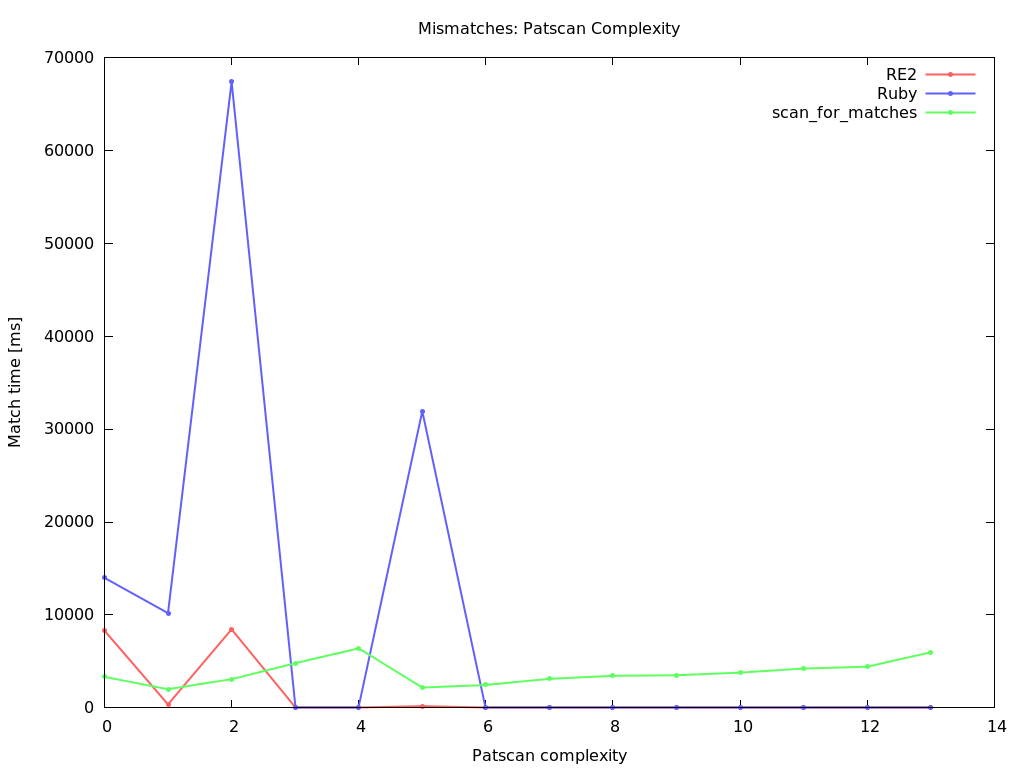
\includegraphics[scale=0.55]{graphs/mismatches.png}	
	\end{center}
	\caption{The results of tests with patterns containing 1, 2, 3, or 4 mismatches. The graph shows the relationship between the size of the sequence and the amount of time it took to search the input file for the matches.}
	\label{graph:cases:mismatches}
\end{figure}

\subsubsection{Deletions}

For deletions we notice the same trend as with mismatches with respect to RE2. RE2 outperforms SFM, Ruby, python, and PR until it reaches a point where the regular expressions simply become too large and it either slows down or fails. Interestingly RE2 is able to break this trend for three deletions, where we notice a big slowdown with sequence length 12, but a great recovery for sequences of length 13 and 14. We suspect that this is due to fewer matches being found for the greater lengths.

\begin{figure}[H]
	\begin{center}
		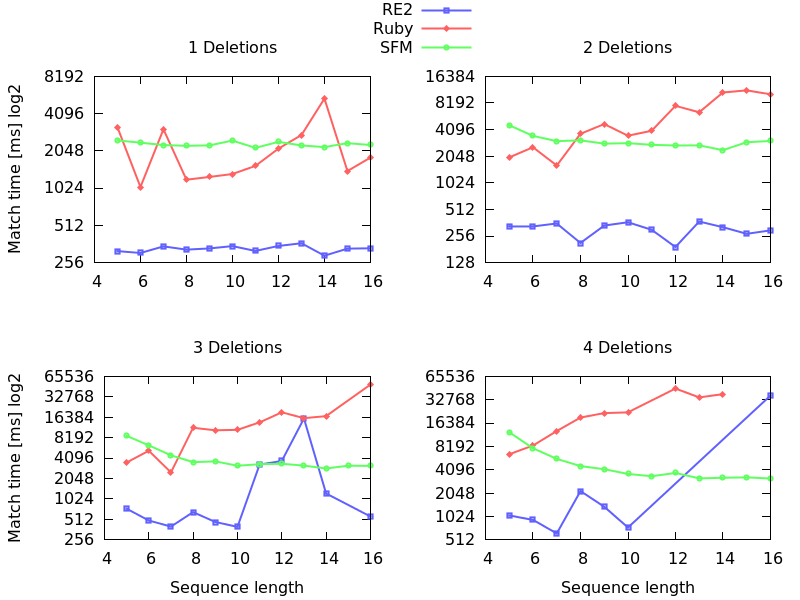
\includegraphics[scale=0.55]{graphs/deletions.png}	
	\end{center}
	\caption{The results of tests with patterns containing 1, 2, 3, or 4 deletions. The graph shows the relationship between the size of the sequence and the amount of time it took to search the input file for the matches.}
	\label{graph:cases:deletions}
\end{figure}


\subsubsection{Insertions}

For insertions we notice a similar trend as before with respect to RE2's relative performance over Ruby and SFM. Since insertions generate much larger regular expressions, we also notice that both Ruby and RE2 are quickly unable to run the expressions. Neither RE2 or Ruby are able to finish sequences with two insertions, failing at 11 and 15 characters respectively.

\begin{figure}[H]
	\begin{center}
		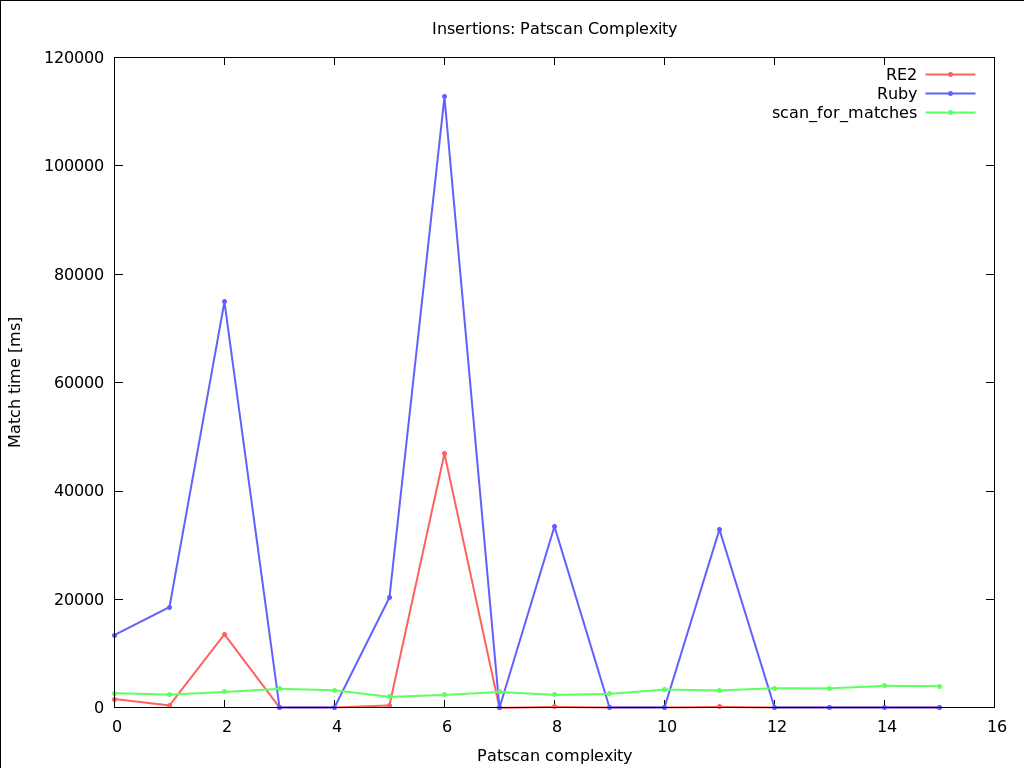
\includegraphics[scale=0.55]{graphs/insertions.png}	
	\end{center}
	\caption{The results of tests with patterns containing 1, 2, 3, or 4 insertions. The graph shows the relationship between the size of the sequence and the amount of time it took to search the input file for the matches.}
	\label{graph:cases:insertions}
\end{figure}

\subsubsection{Mismatches \& Deletions}

For mismatches and deletions we notice that both RE2 and Ruby are unable to parse the regular expressions generated from sequences with more than one mismatch and one deletion. RE2 shows a performance advantage over SFM for one mismatch and one deletion in sequences below 9 characters. For 10 characters and above, RE2 either slows down tremendously or completely fails.

\begin{figure}[H]
	\begin{center}
		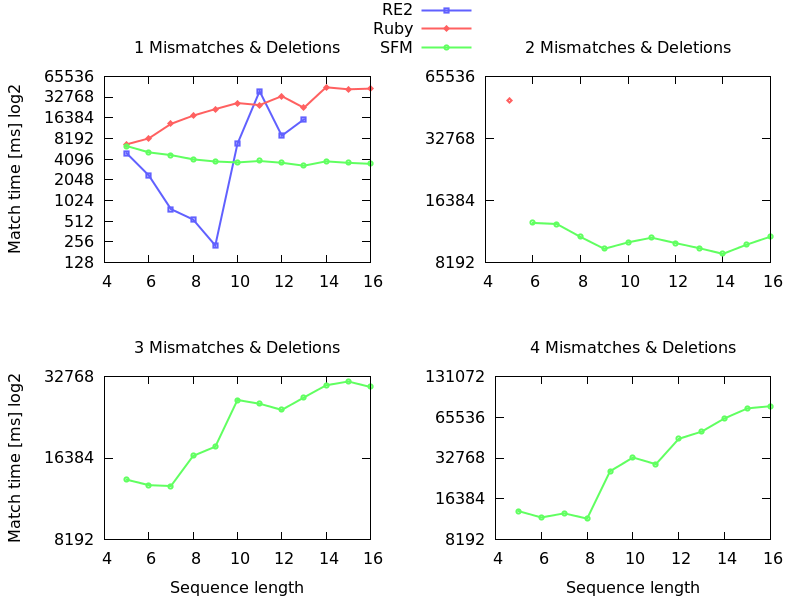
\includegraphics[scale=0.55]{graphs/mismatches_deletions.png}	
	\end{center}
	\caption{The results of tests with patterns containing 1, 2, 3, or 4 mismatches and deletions. The graph shows the relationship between the size of the sequence and the amount of time it took to search the input file for the matches.}
	\label{graph:mismatches:deletions}
\end{figure}

\subsubsection{Mismatches \& Insertions}

For mismatches and deletions we notice a similar trend to that of mismatches and deletions. RE2, Ruby, Python, and PR cannot handle patterns for one mismatch and one insertion of lengths beyond 13, 12, 6, and 13 characters respectively.

An interesting limitation for our regular expressions is also made visible, since we do not have any results for four mismatches and four deletions. This is due to the fact that our implementation at this point exceeds the 8GBs of RAM in our testing computer. 

\begin{figure}[H]
	\begin{center}
		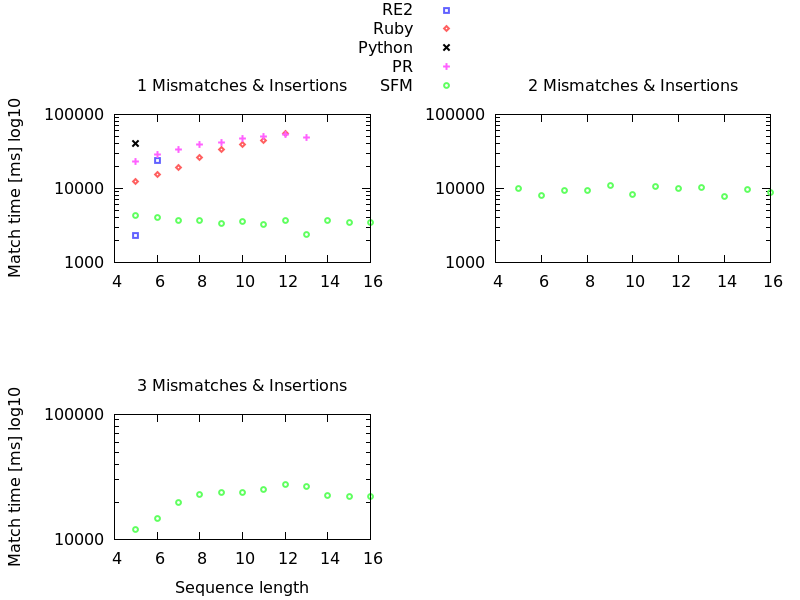
\includegraphics[scale=0.55]{graphs/mismatches_insertions.png}	
	\end{center}
	\caption{The results of tests with patterns containing 1, 2, or 3 mismatches and insertions. The graph shows the relationship between the size of the sequence and the amount of time it took to search the input file for the matches.}
	\label{graph:cases:combinations}
\end{figure}

\subsubsection{Deletions \& Insertions}

For deletions and insertions the trend is again similar to that of mismatches and deletions, and mismatches and insertions. However in this case RE2 fluctuates with regards to match time for one deletion and one insertion. Where it shows a somewhat clear trend of increasing match time in the two other cases mentioned, RE2 in this case is several orders of magnitudes slower than SFM for the sequence of length 8. For sequences of length 9 RE2 is several orders of magnitude faster. Slower again for 11 characters, and faster again for 13 characters.

\begin{figure}[H]
	\begin{center}
		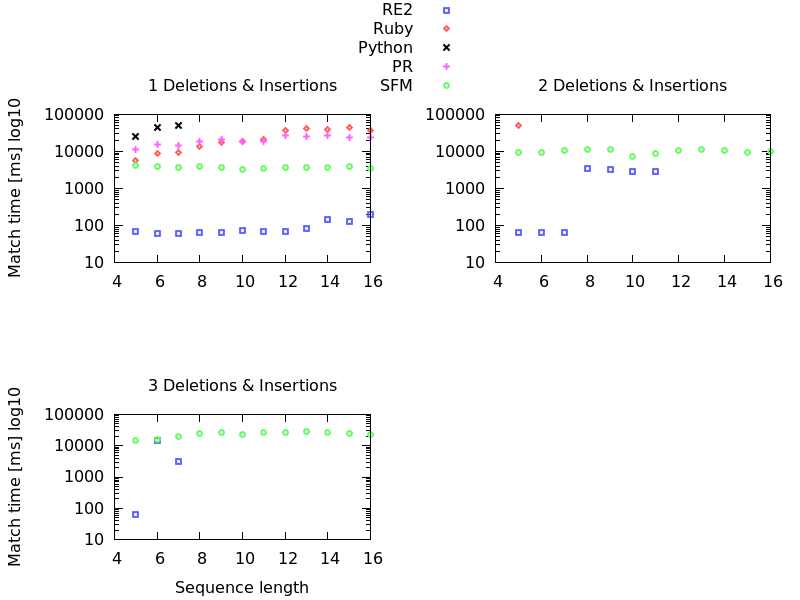
\includegraphics[scale=0.55]{graphs/deletions_insertions.png}	
	\end{center}
	\caption{The results of tests with patterns containing 1, 2, or 3 deletions and insertions. The graph shows the relationship between the size of the sequence and the amount of time it took to search the input file for the matches.}
	\label{graph:cases:combinations}
\end{figure}

\subsubsection{Combinations}

For combinations where we have at least one mismatch, one insertion and one deletion neither RE2, Ruby (except for a single outlier), Python, or PR is able to successfully parse any of the regular expressions generated from the sequences.

\begin{figure}[H]
	\begin{center}
		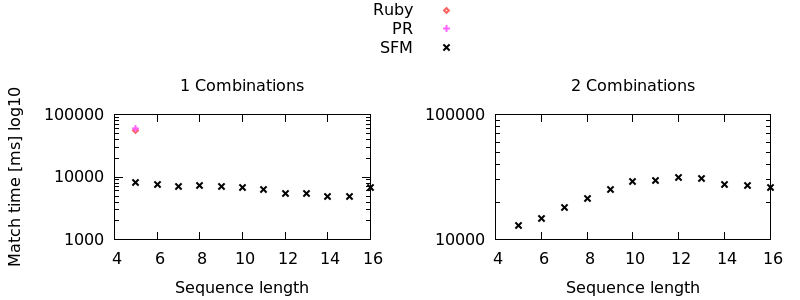
\includegraphics[scale=0.55]{graphs/combinations.png}	
	\end{center}
	\caption{The results of tests with patterns containing 1 or 2 mismatches, deletions, and insertions. The graph shows the relationship between the size of the sequence and the amount of time it took to search the input file for the matches.}
	\label{graph:cases:combinations}
\end{figure}

\subsubsection{Ranges}

Figure~\ref{graph:cases:ranges} shows ranges and how the size of the range affects the match time for all three engines. Contrary to our previous test figures, both RE2 and Ruby shows superior performance to SFM. This is likely caused by the fact that these range patterns are not translated into enormous REs like some of the other patterns. The match time for all three engines are somewhat constant as the size of the range increases. This means that the size of the range does not seem to affect the match time.

PR is clearly the fastest of all three engines, with match times around 13 times faster than SFM. While not as fast as PR; RE2 and Ruby is also performing around 3.5 and 9 times faster than SFM, respectively.

\begin{figure}[H]
	\begin{center}
		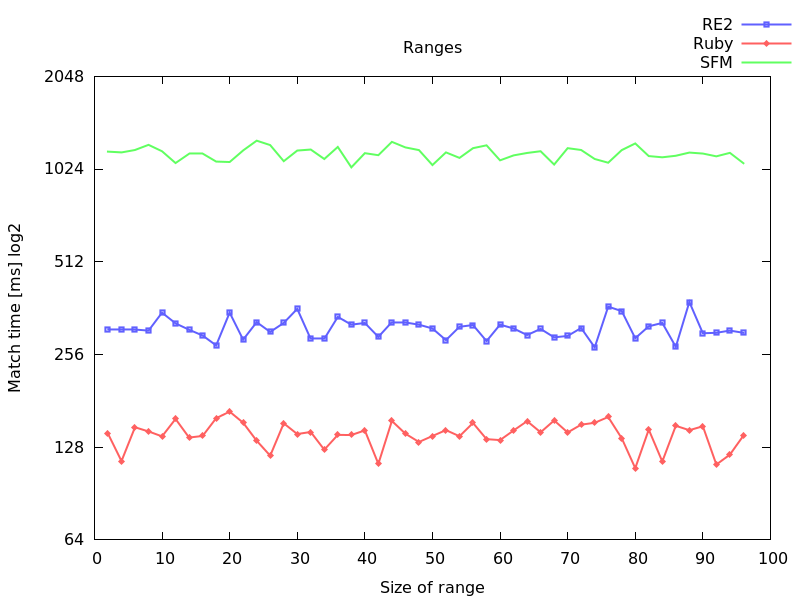
\includegraphics[scale=0.55]{graphs/ranges.png}	
	\end{center}
	\caption{The results of tests with patterns containing ranges of different sizes, where the size of the range \texttt{2...4} is 2 etc. The range has a small sequence on either side, to make sure it doesn't match everything in the input file. The graph shows the relationship between the size of the range, and the amount of time it took to search the input file for matches.}
	\label{graph:cases:ranges}
\end{figure}


\subsubsection{Sequences}

Figure~\ref{graph:cases:sequences} shows patterns containing sequences of different sizes, and how the size of the sequence influences the time it takes all three engines to search the input file for matches.

As with ranges, sequences are simple patterns when translated into REs (In fact, they do not change at all). Figure~\ref{graph:cases:sequences} shows that RE2, Ruby, and PR perform a lot better than SFM. On average, RE2 is about 4 times as fast as SFM, Ruby is matching roughly 8 times as fast, and PR is the fastest with a matching time more than 20 times as fast.

\begin{figure}[H]
	\begin{center}
		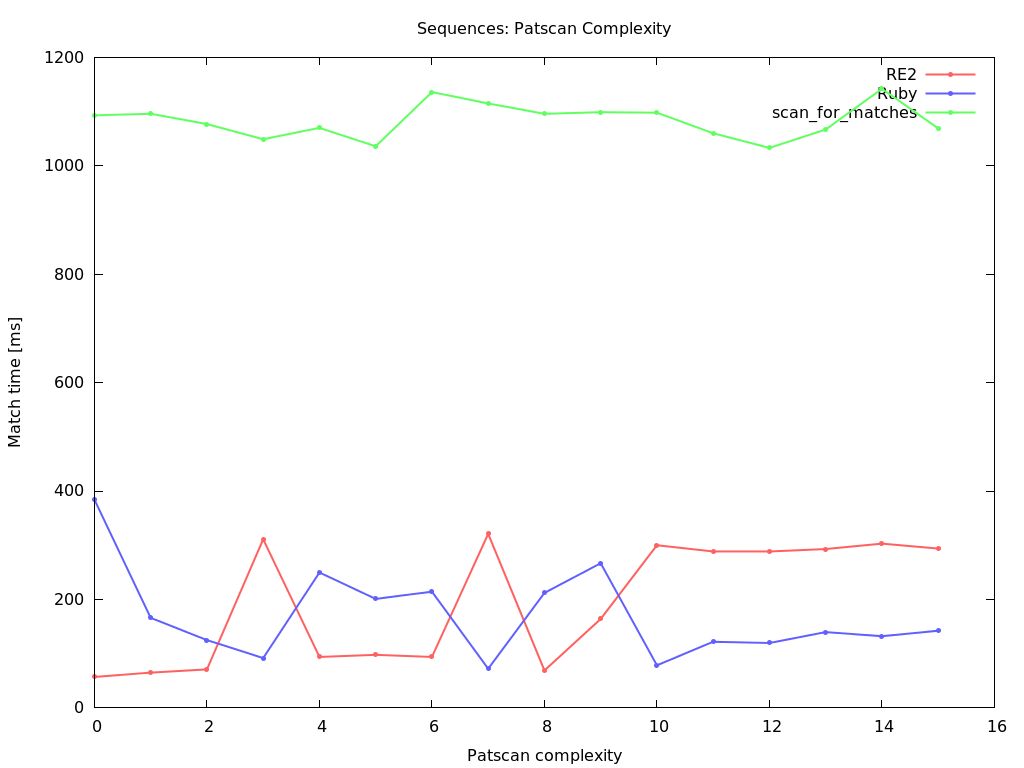
\includegraphics[scale=0.55]{graphs/sequences.png}	
	\end{center}
	\caption{The results of tests with patterns containing sequences of different sizes. The graph shows the relationship between the size of the sequence, and the amount of time it took to search the input file for matches.}
	\label{graph:cases:sequences}
\end{figure}

\section{Conclusion and future work}

We presented a way to translate a significant subset of patscan patterns into regular expressions. By doing so we were able to analyse the performance of SFM against various regular expression implementations, to see if it could prove advantageous to run the patscan patterns searches on regular expression implementations.

Our algorithm proved to be able to translate patterns at very high speeds. Translating patterns takes exponential time, but at a much lower rate than matching the exponentially large REs. Due to this, the time it takes to translate patterns is insignificant compared to the matching time.

From our tests we were able to determine that in a few cases, translating patscan patterns into regular expressions yields better performance than SFM. This happens for very simple patterns, such as sequences, ranges, or very simple combination patterns such as those, where $m+d+i<2$. For some of these patterns, translating into a RE gives a match time more than 4 times faster than SFM.

For a narrow subset of the likely patscan patterns, translating patscan patterns into REs for the purpose of achieving a faster match time is proven to be advantageous. However, for most patterns SFM shows superior match time.

The overall conclusion of the experiment is that translating patscan patterns into REs before matching can only pay off, in terms of performance, in some cases. With this in mind, a hybrid between a RE engine and the SFM engine could be implemented that could run a RE implementation for some patterns, while it runs a SFM-like implementation for other patterns, in order to achieve an overall increase in performance.

While this is certainly possible, a better solution would probably be to not use REs. Instead, a reimplementation of SFM, or another system, specifically designed to search in DNA or protein sequences. Many of the features in REs are not necessary for such an implementation, and disregarding them could lead to better performance.


\newpage

\pagenumbering{gobble}
\bibliographystyle{plain}
\nocite{*}
\bibliography{litterature}

\end{document}
